\chapter{Search Engine}
An \emph{search engine} it comes of several components that can be viewed in figure \ref{img:searchEngine},
we will start talking about crawling and then we will introduce the other components.

In figure \ref{img:bowTie} there is a bow tie that exploits some consideration about crawler where
we can see that web pages that search engine consider are a small amount of all pages. 

\section{Crawling}
Crawling is a graph visit of the web graph, run 24h each days, in order to discover new web pages and we 
have a direct graph $G = (N, E)$ with $N$ that indicate $N$ changes in nodes (usually trillion of nodes) and
$E$ indicate a link between two nodes.

In crawling we have to choose between several issues:
\begin{itemize}
    \item How to crawl? we can choose between quality ("Best" pages first), efficiency (Avoid duplication) and also 
          about malicious pages (Spam pages, Spider traps) including dynamically generated.
    \item How much to crawl and thus index? Coverage and Relative Coverage (coverage comparated with competitor)
    \item How often to crawl? Freshness: How much has changed?
\end{itemize}
Actually is difficult to decide how to implement and design a crawler that should respect the issues that we have
introduced before.

In figure \ref{img:crawler} it is possible to note the general structure of crawler process, in figure \ref{img:crawlerElement} it 
possible to note the component used to implement a crawler and in the end in figure \ref{img:crawlerAlgorithm} there is an pseudocode 
implementation of Crawler's component.

\begin{figure}
    \caption {Diagramm of Crawler operation}
    \label{img:crawler}
    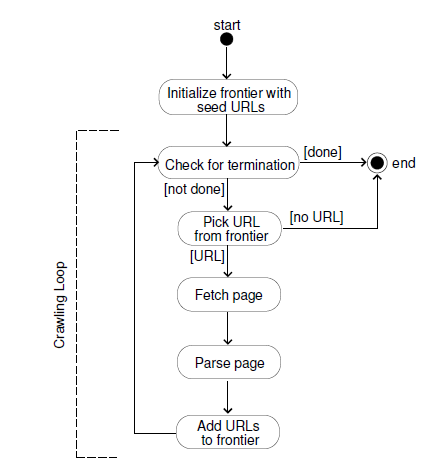
\includegraphics[width=\textwidth]{Images/crawler}
\end{figure}

\begin{figure}
    \caption{Component of Crawler}
    \label{img:crawlerElement}
    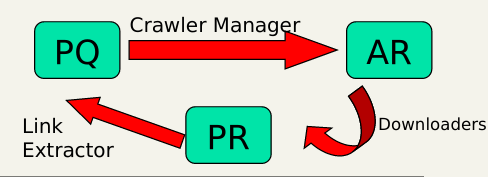
\includegraphics[width=\textwidth]{Images/crawlerComponents}
\end{figure}

\begin{figure}
    \caption{Pseudocode of Crawler components}
    \label{img:crawlerALgorithm}
    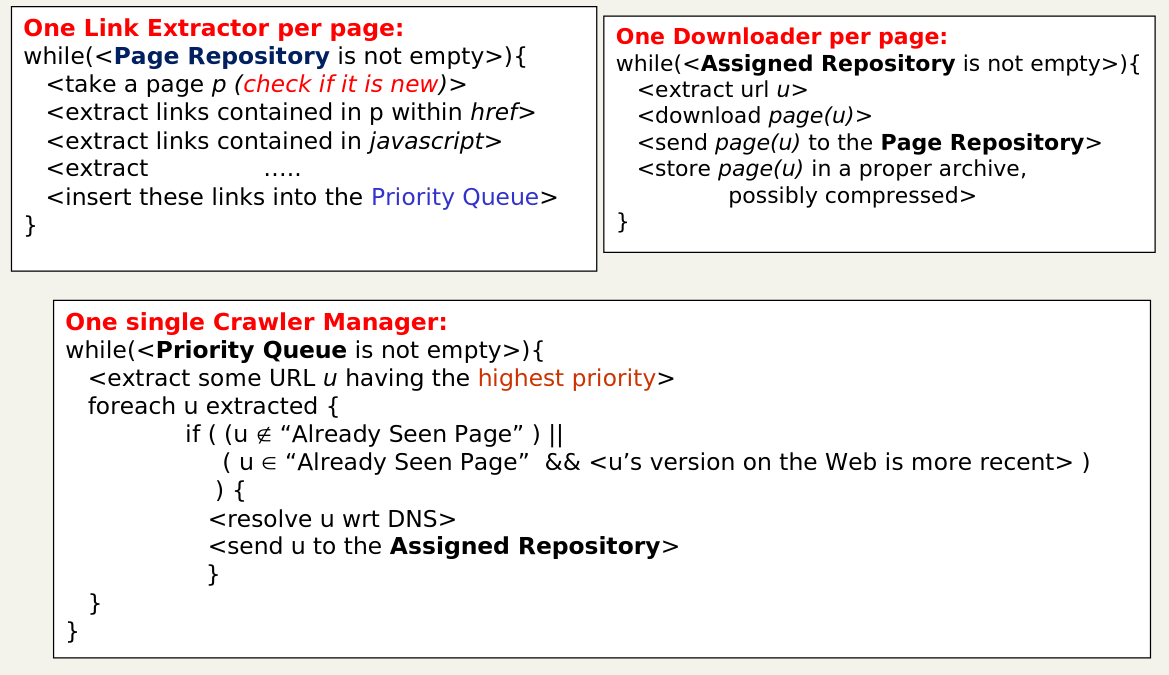
\includegraphics[width=\textwidth]{Images/crawlerPseudocode}
\end{figure}
In visiting the URL frontier we have to define how "good" a page is and there exists several metrics (BFS, DFS, RANDOM, PAGERANK and so on) and also now
we will introduce \emph{Mercator}, an example of search engine released in $1999$, where are present $3$ assumpionts:
\begin{enumerate}
    \item Only one connection per host is open at a time.
    \item a waiting time of a few seconds occurs between successive requests to the same host.
    \item high-priority pages are crawled preferentially.
\end{enumerate}
The structure of Mercator can be viewed in figure \ref{img:mercator} and we have that \emph{Front queues} manage prioritization: prioritizer assigns to an URL an integer priority (refresh,
quality, application specific) between $1$ and $K$ and appends URL to corresponding queue, according to priority.\newline
\emph{Back queues} enforce politeness: each back queue is kept non-empty and contains only URLs from a single host; in a back-queue request it select a front queue randomly, biasing towards higher queues.

\begin{figure}
    \caption{Structure of Mercator search engine}
    \label{img:mercator}
    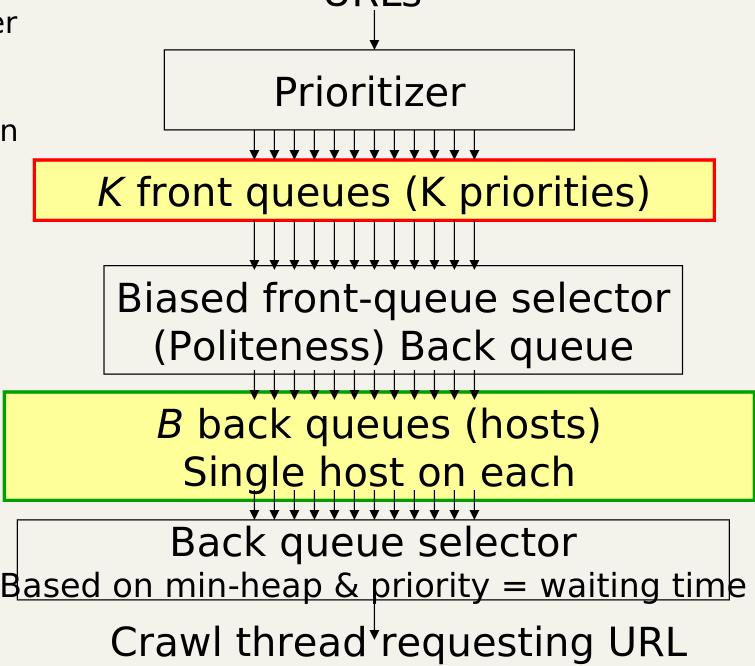
\includegraphics[width=\textwidth]{Images/mercator}
\end{figure}
The \emph{min-heap} contains one entry per back queue and the entry is the earliest time $t_e$ at which the host corresponding to the back queue can be “hit again”:
this earliest time is determined from last access to that host and any time buffer heuristic we choose.\newline
The \emph{crawl thread} consist that a crawler seeks a URL to crawl: extracts the root of the heap, waits the indicate time $t_{url}$, parses URL and adds its out-links to the Front queues.\newline
If back queue $q$ gets empty, pulls a URL $v$ from some front queue (more prob for higher queues): if there’s already a back queue for v’s host, append v to it and 
repeat until q gets not empty, else make q the back queue for v’s host.\newline
If back queue q is non-empty, pick URL and add it to the min-heap with $priority = waiting time t_{url}$.

To check if the page has been parsed/downloaded before URL match, duplicate document match and near-duplicate document match we have several solutions:
\begin{itemize}
    \item Hashing on URLs: after $50$ bln pages, we have “seen” over $500$ bln URLs and each URL is at least $1000$ bytes on average so in overall we have about $500.000 Tb (=500 Pb)$ for just the URLS
    \item Disk access with caching (e.g. Altavista): $>5$ ms per URL check and $>5 ms * 5 * 10^{11}$ URL-checks ($80 years/1PC$ or $30gg/1000 PCs$).
    \item \emph{Bloom Filter} (Archive): for $500$ bln URLs we have about $500 Tbit = 50Tb$
\end{itemize}

\section{Bloom Filter}
An empty Bloom filter is a bit array of $m$ bits, all set to $0$ and there must also be $k$ different hash functions defined, each of which maps or hashes some set element to one of the
$m$ array positions, generating a uniform random distribution.\newline
Typically, $k$ is a small constant which depends on the desired false error rate $\epsilon$, while $m$ is proportional to $k$ and the number of elements to be added and 
to add an element, feed it to each of the $k$ hash functions to get $k$ array positions and set the bits at all these positions to $1$.

To query for an element (test whether it is in the set), feed it to each of the $k$ hash functions to get $k$ array positions and if any of the bits at these positions is $0$,
the element is definitely not in the set; if it were, then all the bits would have been set to $1$ when it was inserted and if all are $1$, then either the element is in the set,
or the bits have by chance been set to $1$ during the insertion of other elements, resulting in a false positive.

In a simple Bloom filter, there is no way to distinguish between the two cases, but more advanced techniques can address this problem and 
the requirement of designing $k$ different independent hash functions can be prohibitive for large $k$, so for a good hash function with a wide output,
there should be little if any correlation between different bit-fields of such a hash, so this type of hash can be used to generate multiple "different" hash functions
by slicing its output into multiple bit fields.\newline
Alternatively, one can pass $k$ different initial values (such as $0, 1, \dots, k-1)$ to a hash function that takes an initial value, or add (or append) these values to the key. 

Removing an element from this simple Bloom filter is impossible because there is no way to tell which of the k bits it maps to should be cleared and although setting any one of those
$k$ bits to zero suffices to remove the element, it would also remove any other elements that happen to map onto that bit, so since the simple algorithm provides no way
to determine whether any other elements have been added that affect the bits for the element to be removed, clearing any of the bits would introduce the possibility of false negatives.

One-time removal of an element from a Bloom filter can be simulated by having a second Bloom filter that contains items that have been removed, however, false positives
in the second filter become false negatives in the composite filter, which may be undesirable and in this approach re-adding a previously removed item is not possible,
as one would have to remove it from the "removed" filter.

Assume that a hash function selects each array position with equal probability, so if $m$ is the number of bits in the array, the probability that a certain bit
is not set to $1$ by a certain hash function during the insertion of an element is
\[ 1 - \frac{1}{m} \]
so if $k$ is the number of hash functions and each has no significant correlation between each other, then the probability that the bit is not set to 1 by any of the hash functions is
\[ (1 - \frac{1}{m})^k \]
and using the well-known identity for $e$ we can obtain for large $m$
\[ (1 - \frac{1}{m})^k = ((1 - \frac{1}{m})^m)^{k/m} \approx -e^{k/m} \]
If we have inserted n elements, the probability that a certain bit is still $0$ is 
\[ (1 - \frac{1}{m})^{kn} \approx -e^{kn}{m} = 0.62^{m/n}\]
It minimize prob. error for $k = (m/n) ln 2$and it is advantageous when $(m/n) << (\text{ key-length in bits } + \log n)$

Pattern maching is a set of objects, whose keys are complex and time costly to be compared (URLs, matrices, MP3 and so on) so we use Bloom Filter to
reduce the explicit comparison and it is effective in hierarchical memories (Example on Dictionary matching).

Another example is \emph{Set intersection}, where we have two machines $M_A$ and $M_B$, each storing a set of items $A$ and $B$ and we wish compute $A \cup B$
exchanging small number of bits.\newline
A solution consist to compute $B - A$ by exchanging small amount of bits ($|A| \log \log |B|$), time depending on $B - A$ and with only $1$ communication round and we consider now
\emph{Patricia Tree}, a special variant of the radix binary trie, in which rather than explicitly store every bit of every key, the nodes store only the position of the first bit
which differentiates two sub-trees.\newline
During traversal the algorithm examines the indexed bit of the search key and chooses the left or right sub-tree as appropriate, and an example can be viewed in figure \ref{img:patricia}.

\begin{figure}
	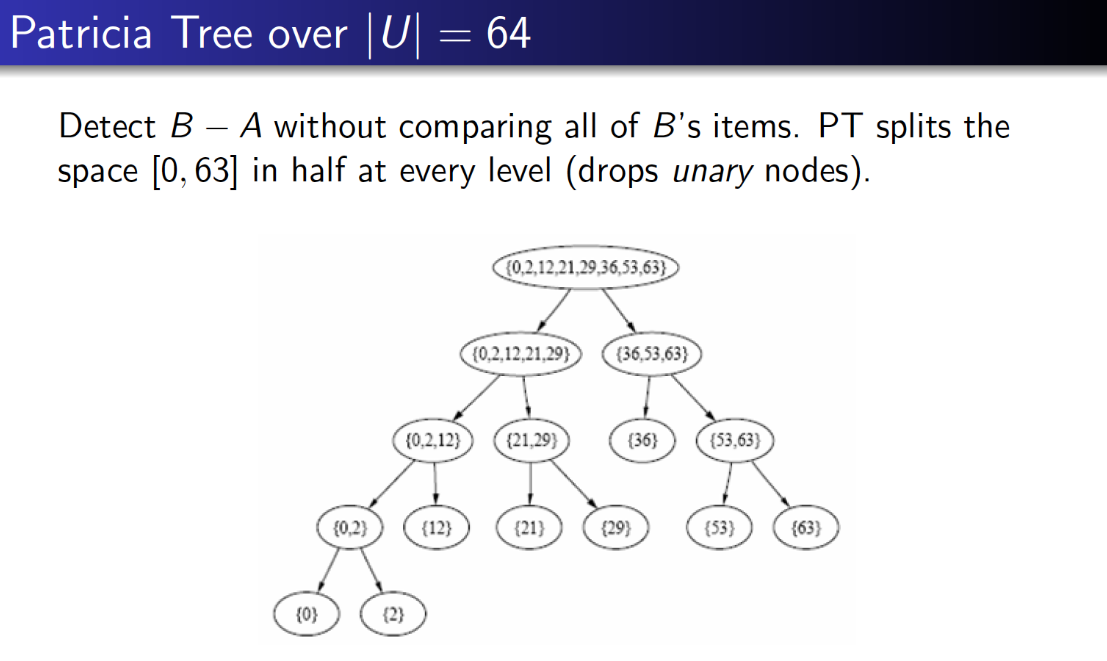
\includegraphics[width=\textwidth]{Images/patricia}
	\caption {Example of Patricia Tree}
	\label{img:patricia}
\end{figure}
Given $PT_A$ and $PT_B$ at machine $M_B$ we procede as follows:
\begin{enumerate}
    \item Visit $PT_B$ top down and compare a node of $PT_B$ against the correspective node in $PT_A$.
    \item If there is a match, the visit backtracks, otherwise proceeds to all children.
    \item If we reach a leaf, then the correspective of $B$ is declared to be in $B - A$
\end{enumerate}
In figure \ref{img:merkleTree} is possible to note Merkle Tree, that are Patricia Tree with hashing and we consider an approximate algorithms, visible in figure \ref{img:approximateAlg},
that use $BF(MT_A)$ to send $MT_A$ in less bits and bookkeeping for its structure, but this of course introduce false-positive errors.
\begin{figure}
	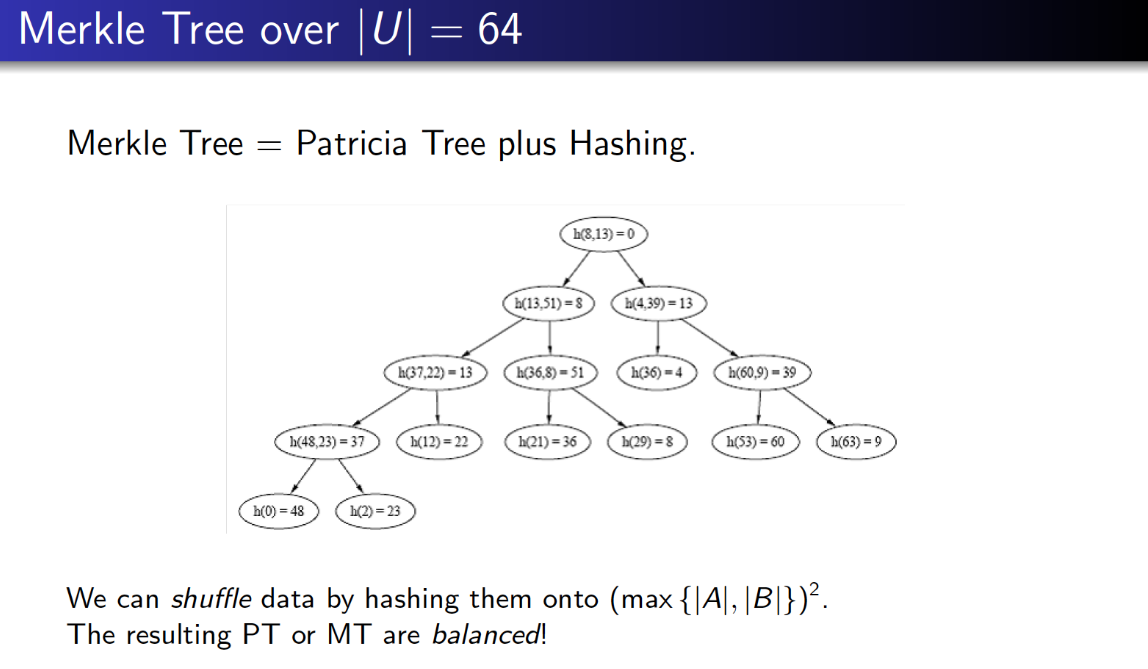
\includegraphics[width=\textwidth]{Images/merkle}
	\caption{Example of Merkle Tree}
	\label{img:merkleTree}
\end{figure}

\begin{figure}
	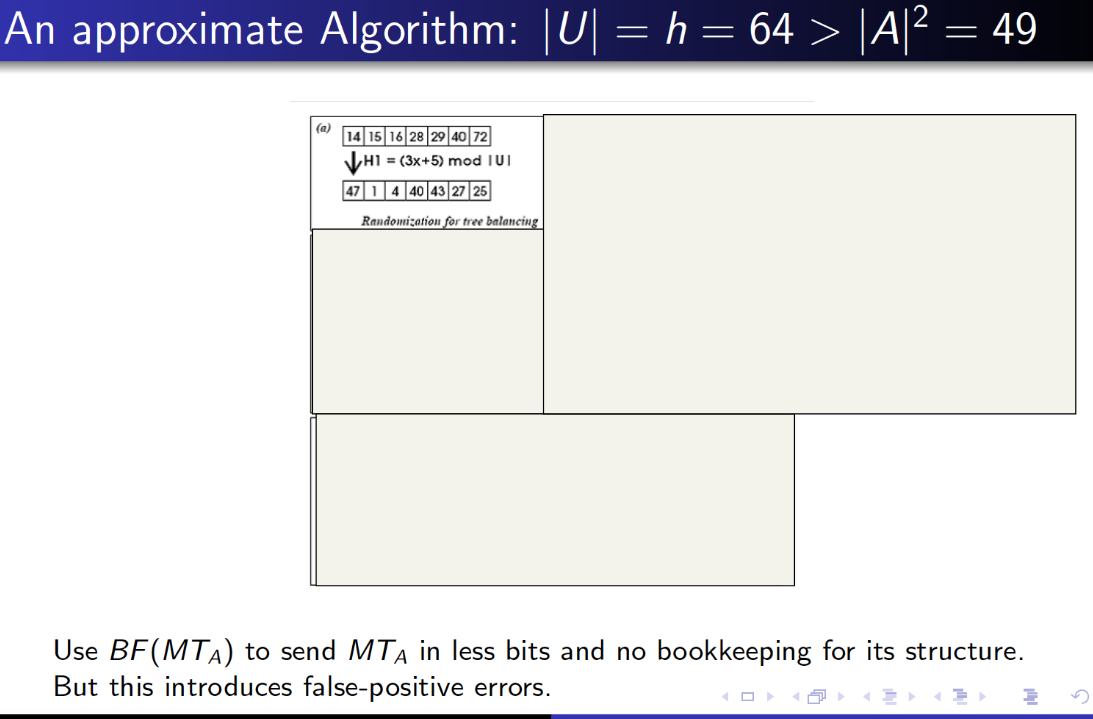
\includegraphics[width=\textwidth]{Images/approximativeAlg}
	\caption{Approximative algorithm to compute Set intersection}
	\label{img:approximateAlg}
\end{figure}
Given $BF(MT_A)$ and $MT_B$, the machine $M_B$ proceeds as follows:
\begin{enumerate}
	\item Visit $MT_B$ top-down and, for each node, check its hash in $BF(MT_A)$.
	\item IF there is a match the visit backtrack, otherwise proceeds to their children.
	\item If we reach a leaf, then the correspective of $B$ is declared to be in $B - A$
\end{enumerate}
Let $m_A = \Theta(|A| \log \log |B|)$ and the optimal $k_A = \Theta(\log \log |B|)$ we send $m_A$ bits for the $BF(A)$ and we have
\[ \epsilon_A = (1/2)^{k_A} = O(1/ \log |B|) \] 
that is the error of $BF(A)$.\newline
The probability of a success for a leaf is given by $(1 - \epsilon_A)^d = \Theta(1)$ and for a correct leaf we have visited its downward path of length $\Theta(\log |B|)$ 
computing $\Theta(\log \log |B|)$ hash functions per node.\newline
This needs a round, $O(|A| \log \log |B|)$ bits, and $O(B - A \log |B| \log \log |B|)$ of reconciliation time.

\subsection{Spectral Bloom Filter}
    We define now an evolution of Bloom Filter, used not only in URL match, with the following definition
    \begin{defi}[Spectral Bloom Filter]
         We have a multiset $M = (S, f_X)$ where $S$ is a multiset and $f_X$ is a count function that return the number of occurrences of $x$ in $M$
    \end{defi}
    Comparated with Bloom Filter we have an slightly large usage of space, but we achieve better performance, and also can be built incrementally for streaming data.

    Applications of this data structure is to answer to two common query:
    \begin{description}
        \item [Iceberg query: ] given $x$ check if $f_X > T$, where $T$ is a dynamically threshold
	\item [Aggregate query: ] $SELECT count(a1) FROM R WHERE a1 = v$
    \end{description}
    B vector is replaced by a vector of counters $C_1, C_2, \dots, C_m$, where $C_i$ is the sum of $f_X$ values for elements $x \in S$ mapping to $i$, and approximations of $f_X$ are stored 
    into $C_{h_1(x)}, C_{h_2(x)}, \dots, C_{h_k(x)}$, but due to conflicts $C_i$ provide only an approximation.

    In figure \ref{img:approximation} is possible to note what is good approximation or a bad approximation of $f_X$, and insertion and deletion are quite simple because we have only
    to increase/decrease each counter by $1$, instead the search operation return the minimum selection (MS) value defined as 
    \[ m_X = \min \{C_{h_1(x)}, \dots, C_{h_k(x)}\} \]

    \begin{figure}
	\caption{Example of approximation between $C_i$ and $f_X$}
	\label{img:approximation}
	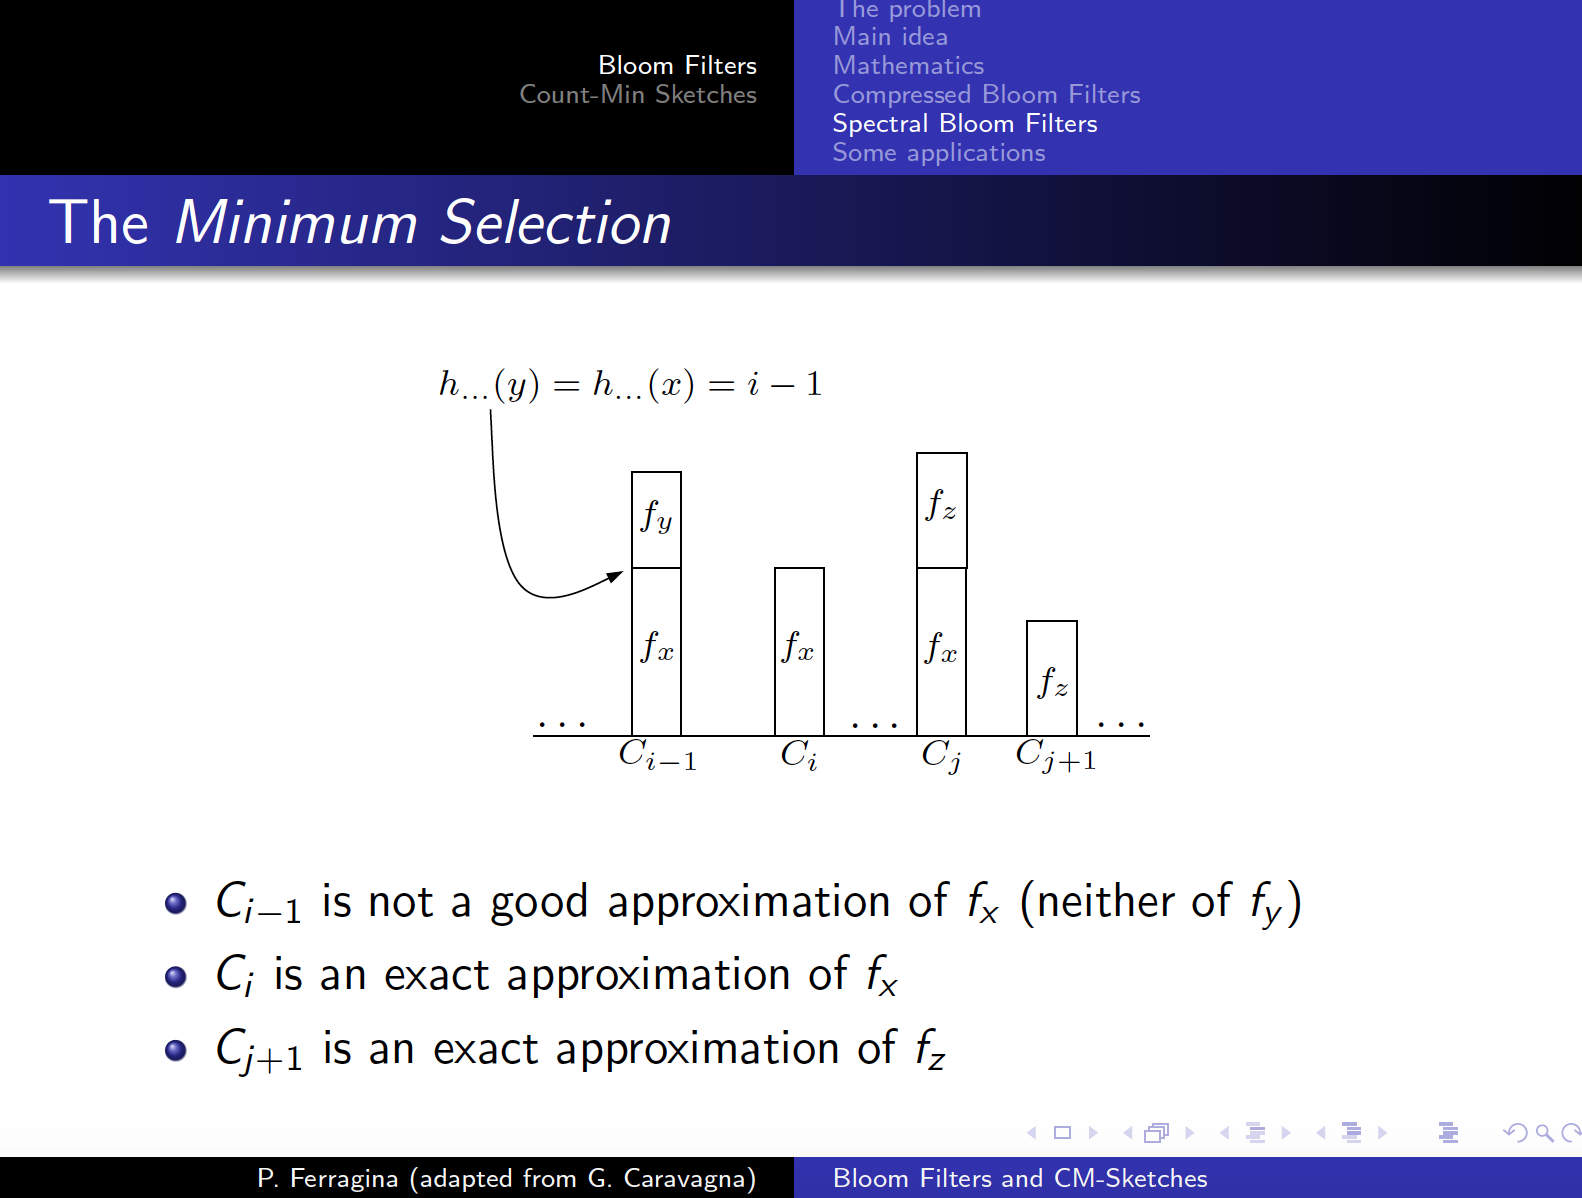
\includegraphics[width=\textwidth]{Images/approximation}
    \end{figure}

    The error rate is the same as bloom filter and we will now prove it 
    \begin{thm}
	For all $x$ it is $f_X \leq m_X$ and we have $f_X \neq m_X$ with probability $E_{SBF} = \epsilon \sim (1-p)^k$
    \end{thm}
    \begin{proof}
	The case that $m_X < f_X$ can not even happen instead the case $m_X > f_X$ happen when all the counter have a collision, that correspond to the event of a false positive in Bloom Filter
    \end{proof}
    Mainly we have two challenges: allow insertion/deletion while we keeping low $E_{SBF}$ and dynamic array of variable-length counters and to solve the first problem we will use \emph{Recurring Minimum (RM)} that is defined as 
    \begin{defi}
	An element has a RM iff more than one of its counters has value equal to the minimum
    \end{defi}
    An item which is subject to a Bloom Error is typically less likely to have recurring minimum among its counters, because we have the following basic idea, using two SBF:
    \begin{enumerate}
	\item For item $x$ with RM we use $m_X$ as estimator, which is highly probable to be correct and hence $E_{SBF_1} < \epsilon$
	\item For items with a SM we use a secondary SBF which is $|SBF_2| << |SBF_1|$ and thus can guarantee $E_{SBF_2} << \epsilon$.
    \end{enumerate}
    With this approach we use more space which could be used for enlarging the single BF, but experiments show that improvements may be remarkable.

    The insertion handles potential future errors, because we increase all counters of $x$ in $SBF_1$ and if $x$ has a $SM$ in $SBF_1$ we look for $x$ in $SBF_2$ and 
    if yes we increase all counters of $x$ in $SBF_2$, otherwise we set $x$ in $SBF_2$ to be the minimum value in $SBF_1$.

    The deletion is the inverse of insertion, so we decrease all counters of $x$ in $SBF_1$ and if $x$ has a SM in $SBF_1$ we decrease all counters of $x$ in $SBF_2$.

    In lookup we have that if $x$ has a RM in $SBF_1$ we return it otherwise we set $m_x^2$ as the value of $x$ in $SBF_2$ that if it is $> 0$ we return it otherwise we return the min value of $x$ in $SBF_1$.


\section{Parallel Crawlers}
    Web is too big to be crawled by a single crawler, work should be divided avoiding duplication so we need several crawlers that works in parallel and assignment 
    between different crawlers can be done in two ways:
    \begin{description}
	    \item [Dynamic assignment: ] central coordinator dynamically assigns URLs to crawlers and it needs communication between coordinator/crawl threads.
	    \item [Static assignment: ] web is statically partitioned and assigned to crawlers and crawler only crawls its part of the web, no need of coordinator and thus communication
    \end{description}
    The Dynamic assignment is problematic because it is computationally expensive and may be complicated, anyway also static assignment has two problem:
    \begin{itemize}
	\item Load balancing the number of URL assigned to crawler because static schemas based on hosts may fail and dynamic assignment may be complicated
	\item Managing the fault-tolerance so in case we have a death of crawler or we have a new crawler we have to recompete the hash function and choose which crawler to assign.
    \end{itemize}
    A nice technique to solve this problem consist in \emph{consistent hashing}, a tool for Spidering, Web Cache, P2P, Routers Load Balance and Distributed FS.\newline
    It consist that item and servers are mapped to unit circle via hash function ID() and item $K$ are assigned to first server $N$ such that $ID(N) \geq ID(K)$, as we can 
    see in figure \ref{img:consistentHashing}.\newline
    Each server gets replicated $\log S$ times, adding a new server moves points between an old server to the new one, only, we have that in average a server gets $\frac{n}{s}$ element.

    \begin{figure}
	\caption{Consistent Hashing Example}
	\label{img:consistenHashing}
	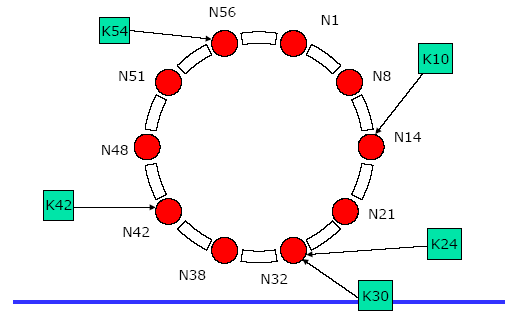
\includegraphics[width=\textwidth]{Images/consistentHashing}
    \end{figure}


\section{Compressed storage of Web Graph}
    Given a directed graph $G = (V, E)$, where $V$ are URLs and $E = (u, v)$ if $u$ has an hyperlink to $v$, also isolated URLs are ignored (they do not have IN and/or OUT)
    and we have three key properties:
    \begin{description}
	    \item [Skewed distribution: ] probability that a node has $x$ links is $1/x^{\alpha}$ with $\alpha \approx 2.1$, so in-value degree follows power law distribution, 
		    			  as we can see in figure \ref{img:altavistaCrawl} and \ref{img:webbaseCrawl}.

					  \begin{figure}
						  \caption{In-degree value in Altavista Crawl in 1997}
						  \label{img:altavistaCrawl}
						  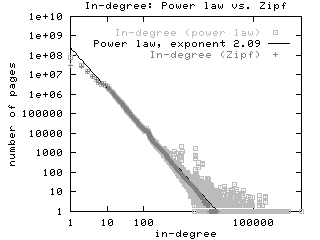
\includegraphics[width=\textwidth]{Images/altavistaCrawl}
					  \end{figure}

					  \begin{figure}
						  \caption{In-degree value in WebBase crawl in 2001}
						  \label{img:webbaseCrawl}
						  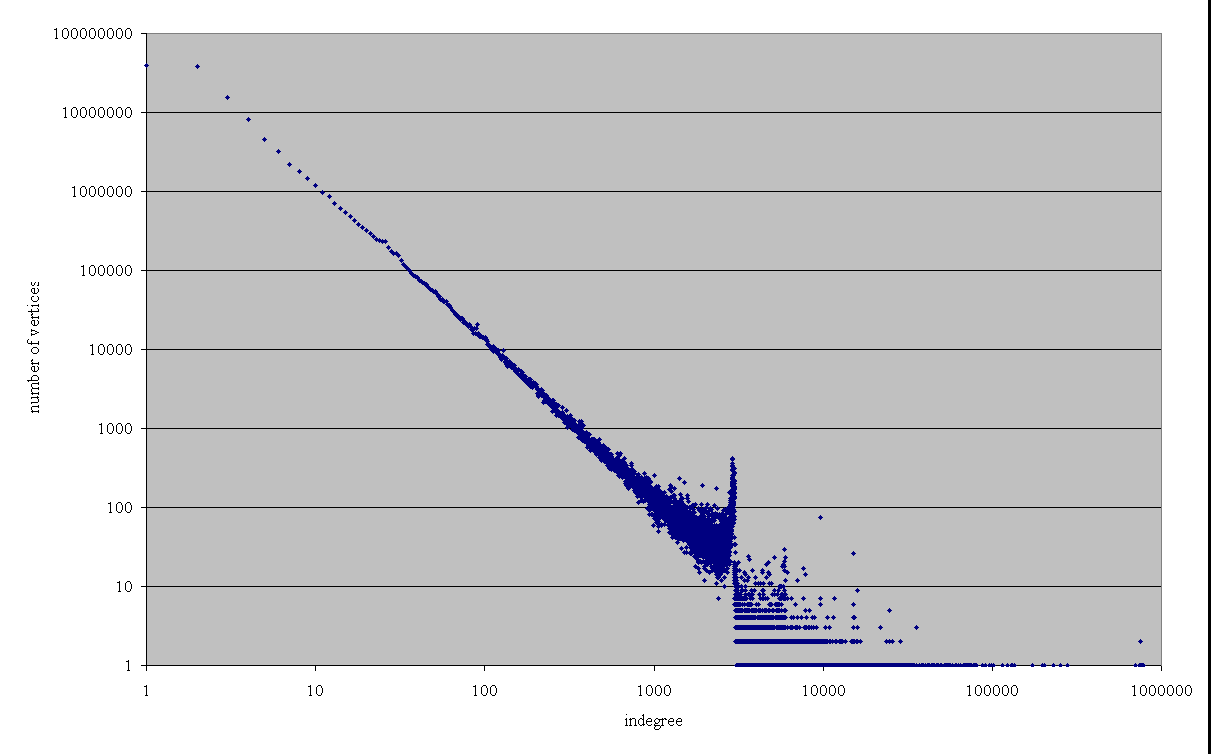
\includegraphics[width=\textwidth]{Images/webBaseCrawl}
					  \end{figure}
						  
	    \item [Locality: ] usually, most of the hyperlinks from URL $u$ point to other URLs that are in the same host of $u$ (about $80\%$), so hosts in the same domain are 
		               close to each other in the lexicographically sorted order, and thus they get close docIDs.

	    \item [Similarity: ] if URLs $u$ and $v$ are close in lexicographic order, then they tend to share many hyperlinks, so we have that each bit of the copy list informs 
		                 whether the corresponding successor of $y$ is also a successor of the reference $x$ and the reference index is the one in $[0, W]$ that gives the best compression,
				 as we can see in figure \ref{img:copyList}.

				 \begin{figure}
					\caption{Example of Copy List}
					\label{img:copyList}
					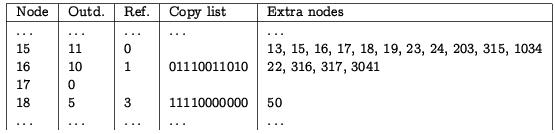
\includegraphics[width=\textwidth]{Images/compressedAdjancency}
				 \end{figure} 
    \end{description}
    To consider these properties we now introduce \emph{copy lists}, to compress information and exploits locality and similarity, but also consider the \emph{copy block}, 
    visible in figure \ref{img:copyBlock}, where the first bit specifies the first copy block and last block is omitted because we know the length from $Out_d$.

    \begin{figure}
	\caption{Example of Copy Block}
	\label{img:copyBlock}
	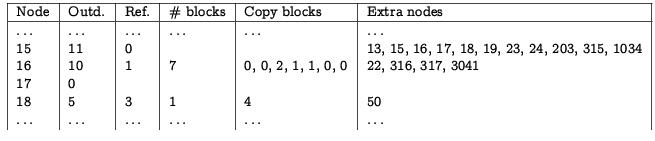
\includegraphics[width=\textwidth]{Images/copyBlock}
    \end{figure}

\section{Locality-sensitive hashing and its applications}
    Given $U$ users, described with a set of d features, the goal is to find (the largest) group of similar users, and to find these group we have three approaches:
    \begin{enumerate}
	\item Try all groups of users and, for each group, check the (average) similarity among all its users.\newline
	      The problem of this approach is that it requires $2^U * U^2$ and also if we limit groups to have a size $\leq L$ we have anyway $U^L * L^2$ 
	      that is computationally infeasible with large $U$.

	\item Interpret every user as a point in a $d$-dim space, and then apply a clustering algorithm, where each iterations require $K * U$ and iterations are relatively small.\newline
	      This approach is locally optimal, comparing users/points costs $O(d)$ in time and space and iterate $k = 1, \dots, U$ costs $U^3 < U^L$, that are in order of years, so 
	      in $T$ time we can manage $U = T^{1/3}$ users.
	
	\item Generate a fingerprint for every user that is much shorter than d and allows to transform similarity into equality of fingerprints.\newline
	      It is randomized, correct with high probability and it guarantees local access to data, which is good for speed in disk/distributed setting.

	      We consider two vectors $p, q \in \{0, 1\}^d$ and we define the \emph{hamming distance} $D(p, q)$ as the number of bits where $p$ and $q$ differ;
	      we define also a \emph{similarity} measure as 
	      \[ s(p, q) = s = \frac{d - D(p, q)}{d} \quad 0 \leq s \leq 1 \]
	      We define now hash functions $h$ by choosing a set $l$ of $k$ random coordinates and we have that the propability to $x$ random such that $p(x) = q(x)$ is defined as 
	      \[ P[\text{picking } x \text{ random such that } p(x) = q(x)] = \frac{d - D(p, q)}{d} = s \]
	      The probability that the hash function $h_I$ has the same value in $p$ and $q$ is defined as 
	      \[ P[h_I(p) = h_I(q)] = s^k = (\frac{d - D(p, q)}{d})^k \]
	      In case we have larger $k$ we have small false positive, instead if we have a large $l$ we have small false negative.

	      We can iterate $L$ times the $k$ projections $h_I(p)$ and we set $g(p) = <h_1(p), h_2(p), \dots, h_L(p)>$, so we declare "$p$ matches $q$" if exist a $I$ such that
	      $h_I(p) = h_I(q)$ and we have that probability of a match defined as 
	       \begin{align}
		      P[g(p) \approx g(q)] & = 1 - P(h_{I_j}(p) \neq h_{I_j}(q) \, \forall j) \\
		                           & = 1 - [P(h_{I_j}(p) \neq h_{I_j}(q)]^L \\
					   & = 1 - (1 - s^k)^L 
	      \end{align} 
	      This probability follow the aspect described in figure \ref{img:matchesProb} and we have that we have to scan all $L$ hash function to create a $L$ fingerprint 
	      with a problem in time complexity.

	      To solve this problem we define for every $p_i$ element $g(p_i) = <h_{I_1}(p_i), h_{I_2}(p_i), \dots, h_{I_L}(p_i)>$ and to compute we follow this algorithm
	     \begin{enumerate}
		\item Sort by $I_1$, scan $g(p_i)$ and find group of continuous vector that have the same first component
		\item Sort by $I_2$, scan $g(p_i)$ and find group of continuos vector that have the same second component
		\item Repeat this approach $L$ times until you sort for $I_L$
	     \end{enumerate}
	     This approach is done by offline search engine, where it is possible to compute statistically connected components, instead online search engine, like databases, 
	     given a query $w$ compute $h_{I_1}(w), \dots, h_{I_L}(w)$ and check the vectors in the buckets $h_J(w)$.

	    This approach of LSH(Locality-sensitive hashing) finds correct clusters with high probability, compares only very short (sketch) vectors, does not need to know the number
	    of clusters and sorts $U$ short items, with few scans.

    \end{enumerate}

\section{Document Duplication}
    The web is full of duplicated content, and exist only few exact duplicate documents but many cases of near duplicates docs (differ for Last modified date, malicious, spam and so on)
    so in this section we will analyze how to determine if two document are duplicates.

   To determine an exact duplication there are several approaches:
   \begin{itemize}
	\item Obvious (slow) technique, like \emph{checksum} (no worst-case collision probability guarantees) or \emph{MD5} (cryptographically-secure string hashes)
	\item Karp-Rabin (fast) scheme: it is a \emph{Rolling hash} (split doc in many pieces), it use arithmetic on primes, it is efficient and has other nice properties.\newline
	      We consider an $m$ bit string $A = 1 a_1 \dots a_{m-1} a_m$ and we choose a prime $p$ in the universe $U$, such that $2p$ uses few memory-words (hence $U \approx 2^64$),
	      so we define the fingerprints $f(A) = A \mod p$, that has a nice properties that if $B = 1 a_2 \dots a_{m-1} a_m a_{m+1}$ we have that 
	      \[ f(B) = [2(A - 2^m - a_1 2^{m-1}) + a_{m+1} + 2^m] \mod p \]
	      and the probabilities that we have a false positive is defined as 
	      \[ \begin{cases}
		      P[\text{false hit to } A \text{ and } B \text{ on same window}] & = \text{Probability } p \text{ divides } (A - B) \\
		                                                                      & = \frac{\# div(A - B)}{\#prime(U)} \\
										      & \approx \frac{(\log (A + B)}{\# prime(U)} \\
										      & = \frac{m \log U}{U} 
		 \end{cases} \]
    \end{itemize}
    Now we consider the problem to given a large collection of documents identify the near-duplicate documents and this aspect is important because it has been found that
    in $1997 30\%$ of web-pages was near-duplicates.


    A common approach used is the \emph{shingling}, where from docs we obtain sets of shingles that are a dissection of document in $q-$gram (shingles), with usually $4 \leq q \leq 8$,
    and the near-duplicate document detection problem reduces to set intersection among integers (shingles), but this naive approaches is computationally expensive so we consider now
    a better approach that use the \emph{Jaccard similarity}, defined as 
    \[ sim(S_A, S_B) = \frac{| A \cap B|}{|A \cup B|} \]
    but also this approach has the problem that we have to compute the similarity of both $A$ and $B$, so a solution consist to use the min hashing, where we define a permutation function,
    we apply them and we take the min element in the permutation of $A$ and $B$.\newline
    An heuristic consist to use $200$ random permutation or pick the $200$ smallest item using only a single permutation, so we obtain a $200$ vector per set which we compare using Hamming distance,
    but of course we can choose how many $k$ element to consider to estimate the Jaccard similarity; the importance of this approximation yields to this important proposition, that will stated and proved
    \begin{prop}
	    $P(\alpha, \beta)$ is exactly the Jaccard similarity $JS(S_A, S_B)$
    \end{prop}
    \begin{proof}
	We give the proof in a slightly more general setting: consider a family of sets whose elements are drawn from a common universe and 
	view the sets as columns of a matrix $A$, with one row for each element in the universe.\newline
	The element $a_{ij} = 1$ if element $i$ is present in the set $S_j$ that the $j$th column represents and let $\Pi$ be a random permutation of  the  rows of $A$;
	denote  by $\Pi(S_j)$ the column that results from applying $\Pi$ to the $j$th column and finally, let $x_{\Pi_j}$ be the index of the first row in which the column
	$\Pi(S_j)$ has a $1$, now we prove that $P(\alpha, \beta) = JS(S_A, S_B)$ and if we can prove this, the theorem follows.

	Consider two columns $j_1, j_2$ and the ordered pairs of entries of $S_{j_1}$ and $S_{j_2}$ partition the rows into four types, as we can note in figure \ref{img:jaccardProof},
	denote by $C_{00}$ the number of rows with $0$’s in both columns, $C_{01}$ the second, $C_{10}$ the third and $C_{11}$ the fourth, then 
	\[ JS(S_{j_1}, S_{j_2}) = \frac{C_{11}}{C_{01} + C_{10} + C_{11}} \]
	To complete the proof by showing that the right-hand side equals to $P(x_{j_1}^{\Pi} = x_{j_2}^{\Pi})$, consider scanning columns $j_1,j_2$ in increasing row
	index until the first non-zero entry is found in either column, and because $\Pi$ is a random permutation, the probability that this smallest row
	has a $1$ in both columns is exactly the right-hand side of Equation.
    \end{proof}
    Another important similarity function is the \emph{cosine Similarity} defined as 
    \[ \cos \alpha = \frac{p * q}{||p|| ||q||} \]
    The computation of the scalar product between $p$ and $q$ is huge, so to solve this problem we use an approximation that consist to construct a random hyperplane $r$ of dimension $d$ and unit norm,
    so we define a sketch vector $h_r(p) = sign(p * r) = \pm 1$ and in a similar way we define a sketch vector for $q$ so we have this proposition
    \begin{prop}
	    $P(h_r(p) = h_r(q)) = 1 - \frac{\alpha}{\pi}$ and also $P(h_r(p) \neq h_r(q)) = \text{hyperplane falls between } p \text{ and } q$
    \end{prop}
    With this probabilistic interpretation we have $O(nk)$ time for each scalar product with an overall time of $O(D * n * k)$, instead if we use $sort(D)$ (I/O efficient) 
    we have $O(D^2)$ that do not scale very well.


